\documentclass[11pt]{article}
\usepackage{mathblatt}

\makeatletter
% Überschrift (Art, Gruppe) im Kasten der nächsten Aufgabe: nie allein am Seitenende (wie \pfab)
\let\gkopf\empty
\newcommand{\gueber}[1]{\gdef\gkopf{#1}}
\newcommand{\gueberdazu}[1]{\ifx\gkopf\empty\gdef\gkopf{#1}\else\expandafter\gdef\expandafter\gkopf\expandafter{\gkopf#1}\fi}
% eingerückt (B6): \gEin Einzug, \gSchrift eine Stufe kleiner; die Überschrift bleibt ohne Einzug
\newlength{\gEin}\setlength{\gEin}{0pt}
\let\gSchrift\relax
% Ankreuzzeile mit hängendem Einzug (lange Aussagen brechen unter dem Text um, nicht unter dem Kästchen)
\renewcommand{\pfkreuzzeile}[1]{\par\noindent\hangindent3.2em\hangafter1\hspace*{1.6em}$\square$\ #1\par}
\RenewDocumentEnvironment{pfaufg}{m m m}{%
  \begin{lrbox}{\mbaufgabebox}\begin{minipage}[t]{\linewidth}%
  \ifx\gkopf\empty\else\noindent\gkopf\par\global\let\gkopf\empty\fi
  \gSchrift\noindent\hspace*{\gEin}\mbpfrandmarke{#1}%
  \begin{minipage}[t]{\mbpfnr}\strut\textbf{#2}\end{minipage}%
  \begin{minipage}[t]{\dimexpr\linewidth-\gEin-\mbpfnr-\mbpfbe\relax}\raggedright\strut\ignorespaces}%
 {\end{minipage}%
  \begin{minipage}[t]{\mbpfbe}\raggedleft\small\color{mbgrau}\strut#3\end{minipage}%
  \end{minipage}\end{lrbox}%
  \setlength{\mbaufgabehoehe}{\dimexpr\ht\mbaufgabebox+\dp\mbaufgabebox\relax}%
  \par\addvspace{6pt}\Needspace*{\mbaufgabehoehe}%
  \noindent\usebox{\mbaufgabebox}\par\addvspace{6pt}}
\makeatother

\begin{document}
\pfheftstil
\fancyfoot[C]{\parbox[t]{\textwidth}{\mbfhbox\par\vspace{1.5mm}{\footnotesize\color{mbgrau}{\scriptsize UTU}\hfill\thepage}}}
\pfheftkopf{Satz des Pythagoras}{P10}
\begin{pfaufg}{}{1.}{}
Kreise den rechten Winkel ein und schreibe H an die Hypotenuse. Hat ein Dreieck keinen rechten Winkel, schreibe „keiner“ darunter.\par\smallskip\noindent \begin{minipage}[t]{0.225\linewidth}\centering 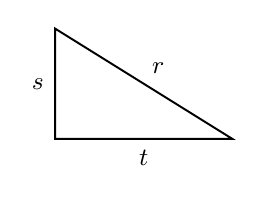
\begin{tikzpicture}[line width=0.7pt,baseline=(current bounding box.north)]\coordinate (P1) at (0.000,0.000);\coordinate (P2) at (2.250,0.000);\coordinate (P3) at (0.000,1.400);\draw (P1) -- (P2) -- (P3) -- cycle;\mbrwmarke{(P1)}{(P2)}{(P3)}\node[font=\small,anchor=south west,inner sep=1.5pt] at (1.167,0.768) {$r$};\node[font=\small,anchor=east,inner sep=1.5pt] at (-0.080,0.700) {$s$};\node[font=\small,anchor=north,inner sep=1.5pt] at (1.125,-0.080) {$t$};\end{tikzpicture}\par\vspace{1mm}{\small a)}\end{minipage}\hfill\begin{minipage}[t]{0.225\linewidth}\centering 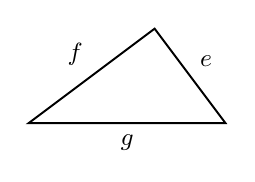
\begin{tikzpicture}[line width=0.7pt,baseline=(current bounding box.north)]\coordinate (P1) at (0.000,0.000);\coordinate (P2) at (2.500,0.000);\coordinate (P3) at (1.600,1.200);\draw (P1) -- (P2) -- (P3) -- cycle;\mbrwmarke{(P3)}{(P1)}{(P2)}\node[font=\small,anchor=south west,inner sep=1.5pt] at (2.114,0.648) {$e$};\node[font=\small,anchor=south east,inner sep=1.5pt] at (0.752,0.664) {$f$};\node[font=\small,anchor=north,inner sep=1.5pt] at (1.250,-0.080) {$g$};\end{tikzpicture}\par\vspace{1mm}{\small b)}\end{minipage}\hfill\begin{minipage}[t]{0.225\linewidth}\centering 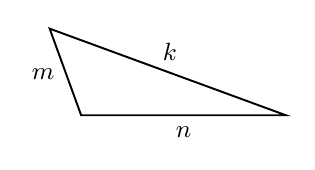
\begin{tikzpicture}[line width=0.7pt,baseline=(current bounding box.north)]\coordinate (P1) at (0.000,0.000);\coordinate (P2) at (2.600,0.000);\coordinate (P3) at (-0.400,1.100);\draw (P1) -- (P2) -- (P3) -- cycle;\node[font=\small,anchor=south,inner sep=1.5pt] at (1.128,0.625) {$k$};\node[font=\small,anchor=east,inner sep=1.5pt] at (-0.275,0.523) {$m$};\node[font=\small,anchor=north,inner sep=1.5pt] at (1.300,-0.080) {$n$};\end{tikzpicture}\par\vspace{1mm}{\small c)}\end{minipage}\hfill\begin{minipage}[t]{0.225\linewidth}\centering 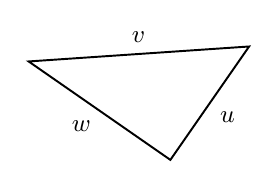
\begin{tikzpicture}[line width=0.7pt,baseline=(current bounding box.north)]\coordinate (P1) at (0.000,1.250);\coordinate (P2) at (1.800,0.000);\coordinate (P3) at (2.800,1.440);\draw (P1) -- (P2) -- (P3) -- cycle;\mbrwmarke{(P2)}{(P1)}{(P3)}\node[font=\small,anchor=north west,inner sep=1.5pt] at (2.366,0.674) {$u$};\node[font=\small,anchor=south,inner sep=1.5pt] at (1.395,1.425) {$v$};\node[font=\small,anchor=north east,inner sep=1.5pt] at (0.854,0.559) {$w$};\end{tikzpicture}\par\vspace{1mm}{\small d)}\end{minipage}
\end{pfaufg}
\par\addvspace{4pt}\begin{center}\begin{minipage}{0.5\linewidth}{\uebersichtskasten{\centering $a^2 + b^2 = c^2$}}\end{minipage}\end{center}\par
\begin{pfaufg}{}{2.}{}
Schreibe die Gleichung erst mit H und K: H² = K² + K². Schreibe sie dann mit den Buchstaben des Dreiecks.\par\smallskip\noindent \begin{minipage}[t]{0.31\linewidth}\centering 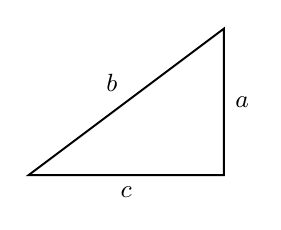
\begin{tikzpicture}[line width=0.7pt,baseline=(current bounding box.north)]\coordinate (P1) at (0.000,0.000);\coordinate (P2) at (2.480,0.000);\coordinate (P3) at (2.480,1.860);\draw (P1) -- (P2) -- (P3) -- cycle;\mbrwmarke{(P2)}{(P1)}{(P3)}\node[font=\small,anchor=west,inner sep=1.5pt] at (2.560,0.930) {$a$};\node[font=\small,anchor=south east,inner sep=1.5pt] at (1.192,0.994) {$b$};\node[font=\small,anchor=north,inner sep=1.5pt] at (1.240,-0.080) {$c$};\end{tikzpicture}\par\vspace{1mm}\raggedright{\small a)}\par\vspace{6mm}\noindent{\color{black!45}\rule{\linewidth}{0.4pt}}\par\vspace{6mm}\noindent{\color{black!45}\rule{\linewidth}{0.4pt}}\end{minipage}\hfill\begin{minipage}[t]{0.31\linewidth}\centering 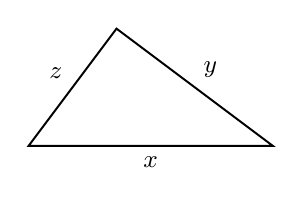
\begin{tikzpicture}[line width=0.7pt,baseline=(current bounding box.north)]\coordinate (P1) at (0.000,0.000);\coordinate (P2) at (3.100,0.000);\coordinate (P3) at (1.116,1.488);\draw (P1) -- (P2) -- (P3) -- cycle;\mbrwmarke{(P3)}{(P1)}{(P2)}\node[font=\small,anchor=south west,inner sep=1.5pt] at (2.156,0.808) {$y$};\node[font=\small,anchor=south east,inner sep=1.5pt] at (0.494,0.792) {$z$};\node[font=\small,anchor=north,inner sep=1.5pt] at (1.550,-0.080) {$x$};\end{tikzpicture}\par\vspace{1mm}\raggedright{\small b)}\par\vspace{6mm}\noindent{\color{black!45}\rule{\linewidth}{0.4pt}}\par\vspace{6mm}\noindent{\color{black!45}\rule{\linewidth}{0.4pt}}\end{minipage}\hfill\begin{minipage}[t]{0.31\linewidth}\centering 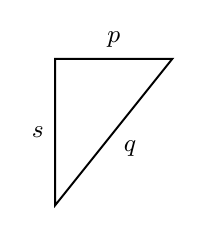
\begin{tikzpicture}[line width=0.7pt,baseline=(current bounding box.north)]\coordinate (P1) at (0.000,0.000);\coordinate (P2) at (0.000,1.860);\coordinate (P3) at (1.488,1.860);\draw (P1) -- (P2) -- (P3) -- cycle;\mbrwmarke{(P2)}{(P1)}{(P3)}\node[font=\small,anchor=south,inner sep=1.5pt] at (0.744,1.940) {$p$};\node[font=\small,anchor=north west,inner sep=1.5pt] at (0.806,0.880) {$q$};\node[font=\small,anchor=east,inner sep=1.5pt] at (-0.080,0.930) {$s$};\end{tikzpicture}\par\vspace{1mm}\raggedright{\small c)}\par\vspace{6mm}\noindent{\color{black!45}\rule{\linewidth}{0.4pt}}\par\vspace{6mm}\noindent{\color{black!45}\rule{\linewidth}{0.4pt}}\end{minipage}
\end{pfaufg}
\par\addvspace{6pt}\gueber{\vspace{10pt}{\large\bfseries Welche Gleichung passt?}\par\vspace{2pt}}
\begin{pfaufg}{nach P10 ’17}{3.}{}
Kreuze die Gleichung an, die für dieses Dreieck gilt:
\par\smallskip\noindent 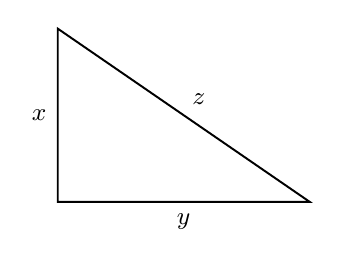
\begin{tikzpicture}[line width=0.7pt,baseline=(current bounding box.north)]\coordinate (P1) at (0.000,0.000);\coordinate (P2) at (3.200,0.000);\coordinate (P3) at (0.000,2.200);\draw (P1) -- (P2) -- (P3) -- cycle;\mbrwmarke{(P1)}{(P2)}{(P3)}\node[font=\small,anchor=south west,inner sep=1.5pt] at (1.645,1.166) {$z$};\node[font=\small,anchor=east,inner sep=1.5pt] at (-0.080,1.100) {$x$};\node[font=\small,anchor=north,inner sep=1.5pt] at (1.600,-0.080) {$y$};\end{tikzpicture}\par
\pfkreuzzeile{$x^2=y^2+z^2$}\pfkreuzzeile{$z^2=x^2-y^2$}\pfkreuzzeile{$z^2\cdot y^2=x^2$}\pfkreuzzeile{$z^2=x^2+y^2$}
\fusshilfe{\mbox{3:~z² = x² + y²}}
\end{pfaufg}
\par\setlength{\gEin}{8mm}\let\gSchrift\small
\begin{pfaufg}{nach P10 ’21}{4.}{}
Kreuze die Formel an, mit der man z berechnet:
\par\smallskip\noindent 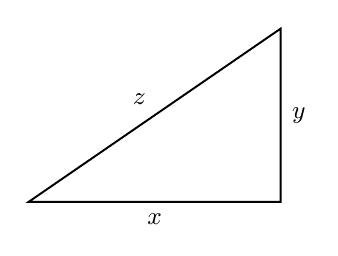
\begin{tikzpicture}[line width=0.7pt,baseline=(current bounding box.north)]\coordinate (P1) at (0.000,0.000);\coordinate (P2) at (3.200,0.000);\coordinate (P3) at (3.200,2.200);\draw (P1) -- (P2) -- (P3) -- cycle;\mbrwmarke{(P2)}{(P1)}{(P3)}\node[font=\small,anchor=west,inner sep=1.5pt] at (3.280,1.100) {$y$};\node[font=\small,anchor=south east,inner sep=1.5pt] at (1.555,1.166) {$z$};\node[font=\small,anchor=north,inner sep=1.5pt] at (1.600,-0.080) {$x$};\end{tikzpicture}\par
\pfkreuzzeile{$z=\sqrt{x^2-y^2}$}\pfkreuzzeile{$z=\sqrt{x^2+y^2}$}\pfkreuzzeile{$z=\sqrt{y^2-x^2}$}\pfkreuzzeile{$z=y^2+x^2$}
\fusshilfe{\mbox{4:~z = √(x² + y²)}}
\end{pfaufg}
\begin{pfaufg}{nach P10 ’26}{5.}{}
Kreuze an, mit welcher Gleichung man w berechnen kann:
\par\smallskip\noindent 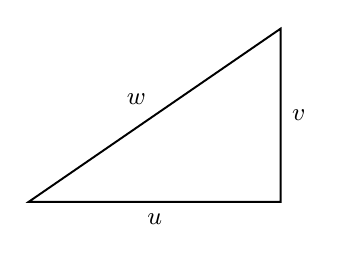
\begin{tikzpicture}[line width=0.7pt,baseline=(current bounding box.north)]\coordinate (P1) at (0.000,0.000);\coordinate (P2) at (3.200,0.000);\coordinate (P3) at (3.200,2.200);\draw (P1) -- (P2) -- (P3) -- cycle;\mbrwmarke{(P2)}{(P1)}{(P3)}\node[font=\small,anchor=west,inner sep=1.5pt] at (3.280,1.100) {$v$};\node[font=\small,anchor=south east,inner sep=1.5pt] at (1.555,1.166) {$w$};\node[font=\small,anchor=north,inner sep=1.5pt] at (1.600,-0.080) {$u$};\end{tikzpicture}\par
\pfkreuzzeile{$w=\sqrt{v^2-u^2}$}\pfkreuzzeile{$w=\sqrt{u^2-v^2}$}\pfkreuzzeile{$w=\sqrt{u^2+v^2}$}
\fusshilfe{\mbox{5:~w = √(u² + v²)}}
\end{pfaufg}
\begin{pfaufg}{nach P10 ’24}{6.}{}
Kreuze die Gleichung an, mit der man die Länge von z berechnen kann:
\par\smallskip\noindent 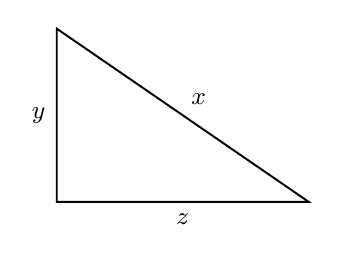
\begin{tikzpicture}[line width=0.7pt,baseline=(current bounding box.north)]\coordinate (P1) at (0.000,0.000);\coordinate (P2) at (3.200,0.000);\coordinate (P3) at (0.000,2.200);\draw (P1) -- (P2) -- (P3) -- cycle;\mbrwmarke{(P1)}{(P2)}{(P3)}\node[font=\small,anchor=south west,inner sep=1.5pt] at (1.645,1.166) {$x$};\node[font=\small,anchor=east,inner sep=1.5pt] at (-0.080,1.100) {$y$};\node[font=\small,anchor=north,inner sep=1.5pt] at (1.600,-0.080) {$z$};\end{tikzpicture}\par
\pfkreuzzeile{$z=x^2-y^2$}\pfkreuzzeile{$z=\sqrt{x^2+y^2}$}\pfkreuzzeile{$z=x+y$}\pfkreuzzeile{$z=\sqrt{x^2-y^2}$}
\fusshilfe{\mbox{6:~z = √(x² $-$ y²)}}
\end{pfaufg}
\begin{pfaufg}{P10 ’22}{7.}{}
Kreuze die Aussage an, die für jedes rechtwinklige Dreieck stimmt:
\pfkreuzzeile{Die Seite gegenüber dem rechten Winkel ist eine Kathete.}\pfkreuzzeile{$c=a+b$}\pfkreuzzeile{Die beiden Kathetenquadrate haben zusammen denselben Flächeninhalt wie das Hypotenusenquadrat}
\end{pfaufg}
\par\setlength{\gEin}{0pt}\let\gSchrift\relax
\par\addvspace{6pt}\gueber{\vspace{10pt}{\large\bfseries Die lange Seite gesucht}\par\vspace{2pt}}
\begin{pfaufg}{}{8.}{}
In einem rechtwinkligen Dreieck sind die Katheten $a = 36$ cm und $b = 15$ cm lang. Berechne die Länge der Hypotenuse $c$.
\par\noindent c² = \leerfeld , c = \leerfeld[cm] \par
\fusshilfe{\mbox{8:~$c = 39$ cm}}
\end{pfaufg}
\begin{pfaufg}{}{9.}{}
In einem rechtwinkligen Dreieck sind $a = 4$ cm und $b = 9$ cm die Katheten. Berechne die Länge der Hypotenuse $c$. Runde auf eine Stelle nach dem Komma.
\par\noindent c² = \leerfeld , c $\approx$ \leerfeld[cm] \par
\fusshilfe{\mbox{9:~$\approx 9{,}8$ cm}}
\end{pfaufg}
\begin{pfaufg}{P10 ’20}{10.}{}
Im Dreieck ABC ist bei C ein rechter Winkel. Die Strecke $\overline{BC}$ ist 12 m lang, die Strecke $\overline{AC}$ 34 m. Berechne die Länge der Strecke $\overline{AB}$.
\par\smallskip\noindent \begin{tikzpicture}[line width=0.7pt,baseline=(current bounding box.north)]\coordinate (P1) at (0.000,0.000);\coordinate (P2) at (1.200,3.400);\coordinate (P3) at (0.000,3.400);\draw (P1) -- (P2) -- (P3) -- cycle;\mbrwmarke{(P3)}{(P1)}{(P2)}\node[font=\small] at (-0.052,-0.295) {$A$};\node[font=\small] at (1.373,3.645) {$B$};\node[font=\small] at (-0.100,3.683) {$C$};\node[font=\scriptsize,mbgrau,anchor=north west] at ([yshift=-2pt]current bounding box.south west) {nicht maßstabsgerecht};\end{tikzpicture}\par
\rechenplatz{2}
\fusshilfe{\mbox{10:~$\overline{AB}$ = 10√13 $\approx$ 36,1 m}}
\end{pfaufg}
\par\setlength{\gEin}{8mm}\let\gSchrift\small
\begin{pfaufg}{nach P10 ’25}{11.}{}
Familie Yücel baut vor der Haustür eine Rampe für Rollstühle. Berechne die Länge x der Rampe.
\par\smallskip\noindent \begin{tikzpicture}[line width=0.7pt,baseline=(current bounding box.north)]\coordinate (P1) at (0.000,0.000);\coordinate (P2) at (5.950,0.000);\coordinate (P3) at (5.950,0.560);\draw (P1) -- (P2) -- (P3) -- cycle;\mbrwmarke{(P2)}{(P1)}{(P3)}\node[font=\small,anchor=west,inner sep=1.5pt] at (6.030,0.280) {16 cm};\node[font=\small,anchor=south,inner sep=1.5pt] at (2.968,0.360) {$x$};\node[font=\small,anchor=north,inner sep=1.5pt] at (2.975,-0.080) {170 cm};\node[font=\scriptsize,mbgrau,anchor=north west] at ([yshift=-2pt]current bounding box.south west) {nicht maßstabsgerecht};\end{tikzpicture}\par
\rechenplatz{2}
\fusshilfe{\mbox{11:~x $\approx$ 170,8 cm}}
\end{pfaufg}
\par\setlength{\gEin}{0pt}\let\gSchrift\relax
\par\addvspace{6pt}\gueber{\vspace{10pt}{\large\bfseries Eine kurze Seite gesucht}\par\vspace{2pt}}
\begin{pfaufg}{}{12.}{}
Leiterlänge und Abstand des Leiterfußes zur Wand sind gegeben, gesucht ist die Höhe an der Wand. Plus oder minus? 
\pfkreuzzeile{Hypotenuse gesucht – plus}\pfkreuzzeile{Kathete gesucht – minus}
\fusshilfe{\mbox{12:~minus}}
\end{pfaufg}
\begin{pfaufg}{}{13.}{}
In einem rechtwinkligen Dreieck ist die Hypotenuse $c = 85$ cm lang. Eine Kathete ist $b = 13$ cm lang. Berechne die Länge der Kathete $a$.
\par\noindent a² = \leerfeld , a = \leerfeld[cm] \par
\fusshilfe{\mbox{13:~$a = 84$ cm}}
\end{pfaufg}
\begin{pfaufg}{}{14.}{}
In einem rechtwinkligen Dreieck ist $c = 11$ cm die Hypotenuse und $b = 6$ cm eine Kathete. Berechne die Länge der Kathete $a$. Runde auf eine Stelle nach dem Komma.
\par\noindent a² = \leerfeld , a $\approx$ \leerfeld[cm] \par
\fusshilfe{\mbox{14:~$\approx 9{,}2$ cm}}
\end{pfaufg}
\begin{pfaufg}{nach P10 ’19}{15.}{}
Amir (A), Ben (B) und Chris (C) spielen sich beim Training den Ball zu. Ermittle den Abstand zwischen Ben und Chris.
\par\smallskip\noindent \begin{tikzpicture}[line width=0.7pt,baseline=(current bounding box.north)]\coordinate (P1) at (0.000,1.600);\coordinate (P2) at (0.000,0.000);\coordinate (P3) at (3.220,0.000);\draw (P1) -- (P2) -- (P3) -- cycle;\mbrwmarke{(P2)}{(P1)}{(P3)}\node[font=\small] at (-0.213,1.811) {$A$};\node[font=\small,anchor=south west,inner sep=1.5pt] at (1.646,0.872) {9 m};\node[font=\small] at (-0.269,-0.133) {$B$};\node[font=\small,anchor=east,inner sep=1.5pt] at (-0.080,0.800) {4 m};\node[font=\small] at (3.511,-0.072) {$C$};\node[font=\scriptsize,mbgrau,anchor=north west] at ([yshift=-2pt]current bounding box.south west) {nicht maßstabsgerecht};\end{tikzpicture}\par
\rechenplatz{2}
\fusshilfe{\mbox{15:~$\overline{BC}$ = √65 $\approx$ 8,06 m}}
\end{pfaufg}
\par\setlength{\gEin}{8mm}\let\gSchrift\small
\begin{pfaufg}{nach P10 ’24}{16.}{}
Eine Seilbahn führt vom Ort B im Tal zum Ort A auf einem Berg. Berechne den Höhenunterschied $\overline{FA}$ zwischen B und A.
\par\smallskip\noindent \begin{tikzpicture}[line width=0.7pt,baseline=(current bounding box.north)]\coordinate (P1) at (0.000,2.870);\coordinate (P2) at (2.550,0.000);\coordinate (P3) at (0.000,0.000);\draw (P1) -- (P2) -- (P3) -- cycle;\mbrwmarke{(P3)}{(P1)}{(P2)}\node[font=\small,anchor=north,inner sep=1.5pt] at (1.275,-0.080) {255 m};\node[font=\small] at (-0.122,3.144) {$A$};\node[font=\small] at (2.811,-0.147) {$B$};\node[font=\small,anchor=south west,inner sep=1.5pt] at (1.335,1.488) {384 m};\node[font=\small] at (-0.199,-0.224) {$F$};\node[font=\scriptsize,mbgrau,anchor=north west] at ([yshift=-2pt]current bounding box.south west) {nicht maßstabsgerecht};\end{tikzpicture}\par
\rechenplatz{2}
\fusshilfe{\mbox{16:~$\overline{FA}$ $\approx$ 287,1 m}}
\end{pfaufg}
\begin{pfaufg}{nach P10 ’26}{17.}{}
Im Parallelogramm ABCD ist die Höhe h eingezeichnet. Berechne die Höhe h.
\par\smallskip\noindent \begin{tikzpicture}[line width=0.6pt,baseline=(current bounding box.north)]\coordinate (A) at (0,0); \coordinate (B) at (3.6,0); \coordinate (F) at (4.9,0); \coordinate (C) at (4.9,2.92); \coordinate (D) at (1.3,2.92);\draw (A)--(B)--(C)--(D)--cycle; \draw[dashed] (B)--(F); \draw[dashed] (C)--(F); \mbrwmarke{(F)}{(C)}{(B)}\node[font=\small,anchor=north east] at (A) {$A$}; \node[font=\small,anchor=north east,inner sep=1pt] at (3.55,-0.05) {$B$}; \node[font=\small,anchor=south west] at (C) {$C$}; \node[font=\small,anchor=south east] at (D) {$D$}; \node[font=\small,anchor=north west] at (F) {$F$};\node[font=\small,anchor=east] at ($(B)!0.5!(C)+(-0.15,0)$) {32 cm}; \node[font=\small,anchor=north,inner sep=1pt] at (4.3,-0.32) {13 cm}; \node[font=\small,anchor=west] at ($(F)!0.5!(C)+(0.12,0)$) {$h$};\node[font=\scriptsize,mbgrau,anchor=north west] at ([yshift=-2pt]current bounding box.south west) {nicht maßstabsgerecht};\end{tikzpicture}\par
\rechenplatz{2}
\fusshilfe{\mbox{17:~h = √855 $\approx$ 29,2 cm}}
\end{pfaufg}
\begin{pfaufg}{nach P10 ’22}{18.}{}
Im Dreieck ABC ist $h_c$ die Höhe auf die Seite $\overline{AB}$. Weise nach, dass die Strecke $\overline{AD}$ etwa 12,0 m lang ist.
\par\smallskip\noindent \begin{tikzpicture}[line width=0.6pt,baseline=(current bounding box.north)]\coordinate (A) at (0,0); \coordinate (D) at (3.6,0); \coordinate (B) at (6.4,0); \coordinate (C) at (3.6,2.22);\draw (A)--(B)--(C)--cycle; \draw[dashed] (C)--(D); \mbrwmarke{(D)}{(C)}{(B)}\node[font=\small,below left] at (A) {$A$}; \node[font=\small,below right] at (B) {$B$}; \node[font=\small,above] at (C) {$C$}; \node[font=\small,below] at (D) {$D$};\node[font=\small,anchor=south east] at ($(A)!0.5!(C)+(-0.08,0.08)$) {14,1 m}; \node[font=\small,anchor=east] at ($(D)!0.3!(C)+(-0.1,0)$) {$h_c \approx 7{,}4$ m};\node[font=\scriptsize,mbgrau,anchor=north west] at ([yshift=-2pt]current bounding box.south west) {nicht maßstabsgerecht};\end{tikzpicture}\par
\rechenplatz{2}
\fusshilfe{\mbox{18:~$\overline{AD}$ = √144,05 $\approx$ 12,0 m}}
\end{pfaufg}
\begin{pfaufg}{P10 ’16}{19.}{}
An einem Fluss liegen der Bioladen C, eine Brücke D und eine Anlegestelle B auf einer Geraden am Ufer. Von einem Ausflugslokal A führt ein 920 m langer Weg zum Bioladen; vom Bioladen bis zur Brücke sind es 541 m. Die Strecke $\overline{AD}$ steht senkrecht auf dem Ufer. Vom Lokal A soll ein neuer Weg direkt zur Brücke D führen. Ermittle die Länge von $\overline{AD}$.
\par\smallskip\noindent \begin{tikzpicture}[line width=0.6pt,baseline=(current bounding box.north)]\coordinate (C) at (0,2.98); \coordinate (D) at (2.16,2.98); \coordinate (B) at (3.6,2.98); \coordinate (A) at (2.16,0);\draw (-0.5,2.98) -- (4.4,2.98); \draw (A)--(C); \draw[dashed] (A)--(D); \mbrwmarke{(D)}{(A)}{(C)}\fill (C) circle (1.2pt); \fill (D) circle (1.2pt); \fill (B) circle (1.2pt); \fill (A) circle (1.2pt);\node[font=\small,above] at (C) {$C$}; \node[font=\small,above] at (D) {$D$}; \node[font=\small,above] at (B) {$B$}; \node[font=\small,below] at (A) {$A$};\node[font=\small,anchor=north east] at ($(A)!0.5!(C)+(-0.1,-0.05)$) {920 m}; \node[font=\small,anchor=north] at ($(C)!0.5!(D)+(0,-0.1)$) {541 m};\node[font=\scriptsize,mbgrau,anchor=west] at (4.4,2.98) {Ufer};\node[font=\scriptsize,mbgrau,anchor=north west] at ([yshift=-2pt]current bounding box.south west) {nicht maßstabsgerecht};\end{tikzpicture}\par
\rechenplatz{2}
\fusshilfe{\mbox{19:~$\overline{AD}$ = √553 719 $\approx$ 744 m}}
\end{pfaufg}
\par\setlength{\gEin}{0pt}\let\gSchrift\relax
\par\addvspace{6pt}\gueber{\vspace{10pt}{\large\bfseries Das Dreieck erst finden}\par\vspace{2pt}}
\begin{pfaufg}{}{20.}{}
Die Figur zeigt ein gleichschenkliges Trapez mit seiner Höhe. Fahre das rechtwinklige Dreieck aus Höhe, Schenkel und Überstand farbig nach. Schreibe dazu, welche Seiten Katheten sind und welche die Hypotenuse ist.
\par\smallskip\noindent \trapez[hoehe=h]{5}{3}{2.5}\par
\rechenplatz{1}
\end{pfaufg}
\begin{pfaufg}{}{21.}{}
Die Figur zeigt ein gleichschenkliges Dreieck. Die Grundseite ist $32$ cm lang, die Schenkel sind je $65$ cm lang. Berechne die Höhe $h$.
\par\smallskip\noindent \begin{tikzpicture}[line width=0.7pt,baseline=(current bounding box.north)]\coordinate (P1) at (0.000,0.000);\coordinate (P2) at (2.290,0.000);\coordinate (P3) at (1.145,4.500);\draw (P1) -- (P2) -- (P3) -- cycle;\node[font=\small,anchor=west,inner sep=1.5pt] at (1.795,2.270) {$65$ cm};\node[font=\small] at (-0.182,-0.238) {$A$};\node[font=\small] at (2.472,-0.238) {$B$};\node[font=\small,anchor=north,inner sep=1.5pt] at (1.145,-0.080) {$32$ cm};\node[font=\small] at (1.145,4.800) {$C$};\coordinate (H) at (1.145,0.000); \draw[dashed,line width=0.5pt] (P3) -- (H); \mbrwmarke{(H)}{(P2)}{(P3)}\node[font=\small,anchor=west] at ($(H)!0.45!(P3)+(0.06,0)$) {$h$};\end{tikzpicture}\par
\par\noindent h² = \leerfeld , h = \leerfeld[cm] \par
\fusshilfe{\mbox{21:~$h = 63$ cm}}
\end{pfaufg}
\begin{pfaufg}{$\bigstar$\,nach P10 ’26}{22.}{}
Ein Turm besteht aus einem Zylinder mit einem Kegeldach. Bestimme die Gesamthöhe des Turms.
\par\smallskip\noindent \begin{tikzpicture}[line width=0.6pt,baseline=(current bounding box.north)]\draw (-0.6,0) -- (-0.6,3.0); \draw (0.6,0) -- (0.6,3.0);\draw (-0.6,0) arc (180:360:0.6cm and 0.18cm); \draw[dashed,line width=0.4pt] (-0.6,0) arc (180:0:0.6cm and 0.18cm);\draw (-0.6,3.0) arc (180:360:0.6cm and 0.18cm); \draw[dashed,line width=0.4pt] (-0.6,3.0) arc (180:0:0.6cm and 0.18cm);\draw (-0.6,3.0) -- (0,3.86) -- (0.6,3.0); \draw[dashed,line width=0.4pt] (0,0) -- (0.6,0); \fill (0,0) circle (0.8pt);\node[font=\small,anchor=north] at (0.3,-0.22) {$r = 4{,}7$ m}; \node[font=\small,anchor=west] at (0.72,1.5) {$h = 25{,}0$ m};\node[font=\small,anchor=south west] at (0.36,3.5) {$s = 8{,}6$ m};\node[font=\scriptsize,mbgrau,anchor=north west] at ([yshift=-2pt]current bounding box.south west) {nicht maßstabsgerecht};\end{tikzpicture}\par
\rechenplatz{3}
\fusshilfe{\mbox{22:~Gesamthöhe $\approx$ 32,2 m}}
\end{pfaufg}
\begin{pfaufg}{nach P10 ’19}{23.}{}
Die Punkte A, B und C bilden ein Dreieck. Berechne die Länge der Strecke $\overline{BC}$.
\par\smallskip\noindent \begin{tikzpicture}\begin{axis}[xmin=-1,xmax=3,ymin=-3,ymax=3,axis lines=middle,tick label style={font=\scriptsize},clip=true,/pgf/number format/use comma,axis line style={-{Stealth[length=2mm]}},every axis plot/.append style={line width=0.9pt},x=0.9cm,y=0.9cm,xtick distance=1,ytick distance=1,enlargelimits=false,grid=both,grid style={mbgitter,line width=0.3pt},major grid style={mbgitter},minor tick num=1,xlabel={$x$},ylabel={$y$},x label style={anchor=west},y label style={anchor=south}]\draw[line width=0.8pt] (axis cs:0,-2) -- (axis cs:2,-2) -- (axis cs:0,2) -- cycle;\fill (axis cs:0,-2) circle (1.6pt) node[above right,font=\small,inner sep=1pt] {$A$};\fill (axis cs:2,-2) circle (1.6pt) node[above right,font=\small,inner sep=1pt] {$B$};\fill (axis cs:0,2) circle (1.6pt) node[above right,font=\small,inner sep=1pt] {$C$};\end{axis}\end{tikzpicture}\par
\rechenplatz{4}
\fusshilfe{\mbox{23:~$\overline{BC}$ = √20 $\approx$ 4,47}}
\end{pfaufg}
\gueberdazu{\vspace{4pt}{\bfseries\small Länge halbieren oder verdoppeln}\par}
\begin{pfaufg}{nach P10 ’15}{24.}{}
Mia baut das Modell einer Pyramide mit quadratischer Grundfläche: Die Grundkante ist 0,80 m lang, die Pyramide ist 0,68 m hoch. Berechne die Höhe einer Seitenfläche.
\rechenplatz{3}
\fusshilfe{\mbox{24:~$h_s$ $\approx$ 0,79 m}}
\end{pfaufg}
\par\setlength{\gEin}{8mm}\let\gSchrift\small
\begin{pfaufg}{nach P10 ’25}{25.}{}
Ein Drachenviereck ABCD hat die Diagonalen $\overline{AC}$ = 50 cm und $\overline{BD}$ = 80 cm. Berechne die Länge der Seite $\overline{AB}$.
\par\smallskip\noindent \begin{tikzpicture}[line width=0.6pt,baseline=(current bounding box.north)]\coordinate (A) at (-2.2,0); \coordinate (C) at (2.2,0); \coordinate (D) at (0,1.75); \coordinate (B) at (0,-3.85); \coordinate (F) at (0,0);\draw (A)--(B)--(C)--(D)--cycle; \draw[line width=0.4pt] (A)--(C); \draw[line width=0.4pt] (B)--(D); \mbrwmarke{(F)}{(C)}{(D)}\node[font=\small,left] at (A) {$A$}; \node[font=\small,right] at (C) {$C$}; \node[font=\small,above] at (D) {$D$}; \node[font=\small,below] at (B) {$B$}; \node[font=\small,anchor=north east] at (-0.05,-0.05) {$F$};\node[font=\small,anchor=west] at (0.08,1.12) {25 cm};\node[font=\scriptsize,mbgrau,anchor=north west] at ([yshift=-2pt]current bounding box.south west) {nicht maßstabsgerecht};\end{tikzpicture}\par
\rechenplatz{2}
\fusshilfe{\mbox{25:~$\overline{AB}$ $\approx$ 60,4 cm}}
\end{pfaufg}
\begin{pfaufg}{$\bigstar$\,nach P10 ’18}{26.}{}
Ein runder Turm hat 6,4 m Durchmesser und ein Dach in Form eines Kegels; die Höhe des Daches ist bekannt. Beschreibe, wie man die Länge eines Dachbalkens berechnen kann.
\par\smallskip\noindent \begin{tikzpicture}[line width=0.6pt,baseline=(current bounding box.north)]\draw (-1.20,0.00) arc (180:360:1.20 and 0.36);\draw[dashed] (1.20,0.00) arc (0:180:1.20 and 0.36);\draw (-1.2,0) -- (0,2.4) -- (1.2,0);\draw[-{Stealth[length=2mm]},line width=0.4pt] (1.9,1.9) node[right,font=\scriptsize] {Dachbalken} -- (0.5,1.4);\node[font=\scriptsize,mbgrau,anchor=north west] at ([yshift=-2pt]current bounding box.south west) {nicht maßstabsgerecht};\end{tikzpicture}\par
\rechenplatz{2}
\fusshilfe{\mbox{26:~√(3,2² + h²)}}
\end{pfaufg}
\begin{pfaufg}{$\bigstar$\,P10 ’22}{27.}{}
Ein Becher hat die Form eines Zylinders ohne Deckel. Er ist 7 cm hoch und hat den Radius 3,2 cm. Ein Rührstab steht schräg im Becher: Er berührt unten den Rand des Bodens und lehnt oben am gegenüberliegenden Rand. 2 cm des Stabs ragen über den Becher hinaus. Bestimme die Länge des Stabs.
\par\smallskip\noindent \begin{tikzpicture}[line width=0.6pt,baseline=(current bounding box.north)]\draw (-1.10,0.00) arc (180:360:1.10 and 0.33);\draw[dashed] (1.10,0.00) arc (0:180:1.10 and 0.33);\draw (-1.1,0) -- (-1.1,2.4); \draw (1.1,0) -- (1.1,2.4);\draw (0,2.4) ellipse (1.1 and 0.33);\draw[line width=1.6pt] (-0.99,-0.15) -- (1.38,3.15);\node[font=\scriptsize,mbgrau,anchor=north west] at ([yshift=-2pt]current bounding box.south west) {nicht maßstabsgerecht};\end{tikzpicture}\par
\rechenplatz{2}
\fusshilfe{\mbox{27:~√89,96 + 2 $\approx$ 11,5 cm}}
\end{pfaufg}
\par\setlength{\gEin}{0pt}\let\gSchrift\relax
\par\vfill\noindent{\footnotesize\color{black!70}Satz des Pythagoras in der P10 seit 2014: Welche Gleichung passt? 5× · Die lange Seite gesucht 2× · Eine kurze Seite gesucht 5× · Das Dreieck erst finden 6× (je EBR und FOR). Nicht geprüft: Umkehrung, Höhensatz und Kathetensatz. \mbox{$\bigstar$ = nur FOR.}\par\noindent Vorher: Quadrat und Wurzel · Weiter: Seiten und Winkel mit sin, cos, tan · Körper: Mantellinie und Höhe\par}
\end{document}